\begin{figure}[htbp]
    \vspace{-3em}
    \centering
    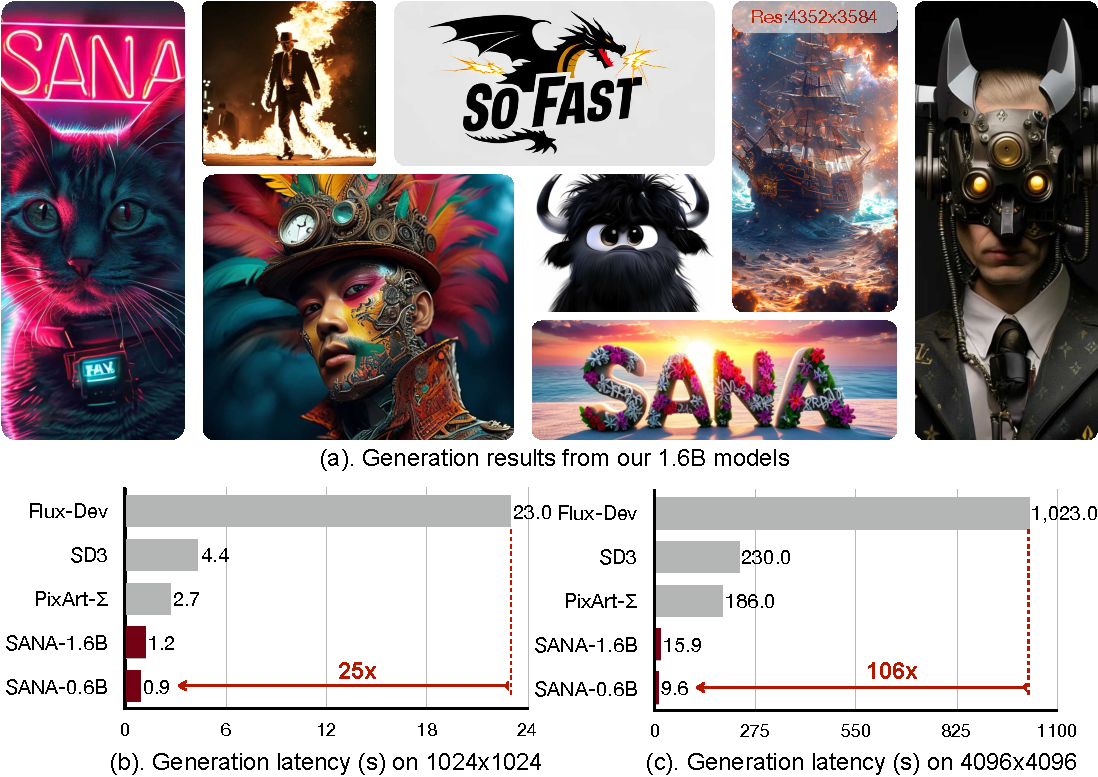
\includegraphics[width=0.90\textwidth]{figures/teaser.pdf}
    % \vspace{-3em}
    \caption{An overview of generated images and inference latency of \methodshort.
    }
    \label{fig:teaser}
\end{figure}

\begin{abstract}
    We introduce \model, a text-to-image framework that can efficiently generate images up to 4096$\times$4096 resolution.
    \model can synthesize high-resolution, high-quality images with strong text-image alignment at a remarkably fast speed, deployable on laptop GPU. 
    Core designs include: 
    (1) Deep compression autoencoder: unlike traditional AEs, which compress images only 8$\times$, we trained an AE that can compress images 32$\times$, effectively reducing the number of latent tokens. 
    (2) Linear DiT: we replace all vanilla attention in DiT with linear attention, which is more efficient at high resolutions without sacrificing quality.
    (3) Decoder-only text encoder: we replaced T5 with modern decoder-only small LLM as the text encoder and designed complex human instruction with in-context learning to enhance the image-text alignment.
    (4)  Efficient training and sampling: we propose Flow-DPM-Solver to reduce sampling steps, with efficient caption labeling and selection to accelerate convergence. 
    As a result, \model-0.6B is very competitive with modern giant diffusion model (e.g. Flux-12B), being 20 times smaller and 100+ times faster in measured throughput. 
    Moreover, \model-0.6B can be deployed on a 16GB laptop GPU, taking less than 1 second to generate a 1024$\times$1024 resolution image.
    Sana enables content creation at low cost. 
    Code and model will be publicly released.
    
\end{abstract}

